\chapter{Transport domain analysis}

In this chapter, we will analyze two variants of the Transport domain: sequential and temporal. To do this, we will describe a system we developed for the analysis
and development of planners for Transport, describe and analyze the datasets
used for devising experiments, and discuss the properties of Transport
that will help us in developing better quality planners.

\section{TransportEditor -- A Transportation Planning System}

To enable effective transportation planning,
we have developed \textit{TransportEditor}, a system for creating and visualizing transportation problems and plans.
Specifically, TransportEditor aims to be a problem editor and plan visualizer for the Transport domain (and its variants). It is an intuitive and cross-platform graphical desktop application (Figure~\ref{fig:transporteditor-screenshot})
written in Java.

It allows the user to create a planning session, where they
select a Transport domain variant, load a problem instance from PDDL (Section~\ref{pddl}) or create a new one from scratch.
The road network of the problem is automatically laid out and visualized for the user as a graph with locations as nodes and roads as edges.
Users can then tweak the layout, make changes to vehicle and package properties
and export the problem or domain back into PDDL.

They can also select an external planner
referencing its executable file, or select one of the built-in planners and try to solve
the loaded problem using the selected planner. Internal and external plan validators, like VAL \citep{Howey2003}, can also be selected to verify plans are correct.
Once plans are loaded and verified, it will let the user see a list of actions
in the plan, or plot a Gantt chart (useful for observing concurrent actions in temporal domain variants).

The best feature of TransportEditor is the option of tracing plans. We can select
any action, specify an exact time point or just step through the actions in order and
the road network on the left will display the current state of the problem, as if
all actions before the current point were applied to the start state.
It is possible to do all of this, and more, without ever leaving the TransportEditor user interface.

TransportEditor will help researchers working on this domain fine-tune their planners; they can visualize the various corner cases their planner fails to handle, step through the generated plan and find the points where their approach fails.
A secondary motivation is to be able to test approaches for creating plans for the domain.
For screenshots of typical TransportEditor usage, see the attached \nameref{transport-editor-screenshots}.

\begin{figure}[t]
\begin{center}
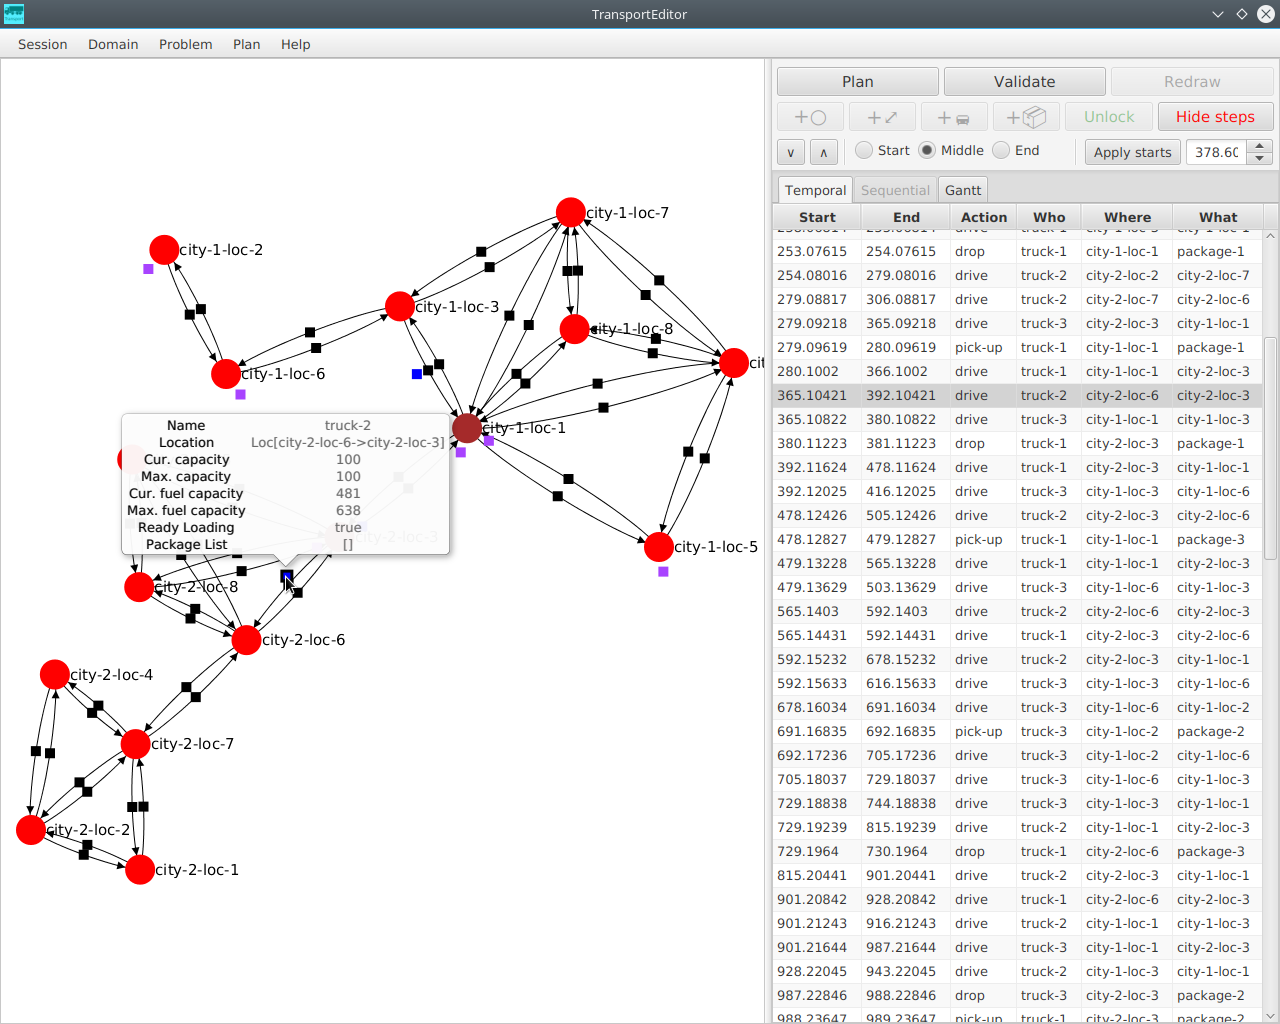
\includegraphics[width=0.9\textwidth]{../img/transporteditor_temporal}
\end{center}
\caption[Screenshot of a user tracing actions of a plan for a small temporal problem in TransportEditor.]{Screenshot of a user tracing actions of a plan for a small temporal problem in TransportEditor. The bubble in the middle shows details
of a truck currently driving along a road between \texttt{city-2-loc-6} and \texttt{city-2-loc-3}. The \texttt{city-1-loc-1} location is plotted in a darker shade of red, which signifies that a petrol station is present at the location.}
\label{fig:transporteditor-screenshot}
\end{figure}

The basic user workflow of TransportEditor consists of the following steps:
\begin{itemize}
\item Selecting which formulation of the Transport domain they want to work with or create their own variant;
\item Loading the PDDL or creating their own problem of the given domain. TransportEditor then visualizes the given graph as good as it can;
\item Iterating among the following options:
\begin{itemize}
\item Loading a planner executable and letting TransportEditor run the planner on the loaded problem instance for a given time (the user can cancel anytime),
then loading the resulting plan;
\item Possibly loading a pre-generated plan;
\item Stepping through the individual plan actions and letting TransportEditor visualize them.
The user can step forward and backward in the plan and inspect each action result in great detail;
\item Editing the graph: adding/removing/editing the location or properties of vehicles, packages, roads, locations and possibly petrol stations;
\item Saving the currently generated plan;
\item Saving the problem;
\item Saving the domain (exporting to a PDDL file).
\end{itemize}
\item Saving and closing the currently loaded problem. Exit the application or go back to the first step.
\end{itemize}

TransportEditor is a part of this thesis and you can find it on the attachment CD (see the attached \nameref{cd-contents} for more information). Both the \nameref{transporteditor-user-manual},
the \nameref{transporteditor-developer-manual}, and the \nameref{transporteditor-developer-javadoc} are attached to this thesis in a digital format, offering guidance when
using the program and providing an in-depth description.
















\section{Properties of Transport domains}

In this section, we will delve more deeply into the Transport domain and try to analyze its properties.
We will describe the problem instances that have been used in the IPC and discuss insights useful for devising heuristics or for other approaches to creating plans for these problems.

\subsection{Does domain knowledge make Transport easy to solve?}

When domain-independent planners solve a sequential Transport problem,
they face a harder task than our planners that have domain knowledge ahead of time.
Deciding whether a plan of a given length exists is, in the case of Transport,
an NEXPTIME-complete task \citep[Section~3.4]{Ghallab2004}.
That does not mean domain knowledge makes Transport easy. We will now show
that even the sequential variant of Transport is NP-hard.

\begin{thm}
The problem of finding an optimal plan for an undirected connected graph in the sequential
Transport domain is NP-hard. \TODO{Formulate better and revise proof}
\end{thm}
\begin{proof}
It is not evident if the problem is in NP: if we get a plan, there is no straightforward
way of verifying whether it is optimal.

We will now show that we can reduce an NP-complete problem to our problem in polynomial time,
hence proving that all NP-complete problems are reducible to our problem,
and therefore, our problem is NP-hard.

As proven by \citet{Karp1972}, the problem of existence of a Hamilton circuit (HC) in a (directed or undirected) graph is NP-complete. We will show that we are able to transform the HC problem into a sequential Transport problem.

Given an undirected graph $G$, the solution to HC is a cycle through all the nodes of $G$,
without visiting any single node twice.
We can use the same graph to model a Transport problem instance.
The problem will contain only one vehicle of capacity $n-1$,
where $n = |G|$, the number of nodes in the graph.

We will co-locate $n-1$ packages with the vehicle at any predetermined graph vertex $l \in G$.
One package $p'$ will be located elsewhere, at $l' \in G,\, l \neq l'$.
Each package positioned at $l$ will have a different target than the other packages at $l$
and none of the targets will be $l$. The package at $l'$ will have the original node $l$
as its target. We will set all road lengths to $1$. 

An optimal plan for the designed translation has a total cost of at least $3n$.
Any plan for this problem has to have at least $n$ \verb+drive+ actions, because
there is a package to be delivered to every node, and the graph has $n$ nodes.
Because it has to move $n$ packages, at least $n$ \verb+pick-up+ and $n$ \verb+drop+
actions are needed. The costs of all actions are 1.
We conjecture that an HC exists if and only if an optimal and valid plan visits each vertex only once.

First, we prove the forward implication. Assume an HC exists and the optimal plan visits at least one node twice. We can now construct a plan with a lower total cost than the optimal plan: first, pick up all the $n-1$ co-located packages, then drive along the HC. At each
visited node, drop the package that has this node as its destination. If we are at $l'$,
pick up the package $p'$. The plan is trivially valid, as it delivers all packages
and the vehicle never over-reaches its capacity. Also, its total cost is $3n$
(the length of the HC is $n$, which implies $n$ drive actions) and for every of the $n$ packages, we do exactly one \verb+pick-up+ and exactly one \verb+drop+. Hence, the plan
is optimal and visits each vertex only once.

Now, assume an HC does not exist. If the found optimal plan only visits each node once,
we can look at the source locations of all \verb+drive+ actions and the target
location of the last \verb+drive+ action. They constitute a path through the graph on which a node never repeats and the path starts and finishes at the same node.
Hence, we have constructed a HC.
\end{proof}


\subsection{Datasets \& problem instances}

For evaluation and comparison with other planners, we have acquired several problem datasets from previous runs of the IPC.
Table~\ref{tab:ipc-datasets} provides an overview of the individual datasets, their associated IPC competition, the track at the competition and the domain variant the problems are modeled in.

\begin{table}[tb]
\begin{tabular}{c||ccc}
\textbf{Dataset} & \textbf{Competition} & \textbf{IPC Track} & \textbf{Formulation} \\ 
\midrule
\midrule
netben-opt-6 & IPC-6 & \href{http://icaps-conference.org/ipc2008/deterministic/NetBenefitOptimization.html}{Net-benefit: optimal} & Numeric \\ 
seq-opt-6 & IPC-6 & \href{http://icaps-conference.org/ipc2008/deterministic/SequentialOptimization.html}{Sequential: optimal} & STRIPS \\ 
seq-sat-6 & IPC-6 & \href{http://icaps-conference.org/ipc2008/deterministic/SequentialSatisficing.html}{Sequential: satisficing} & STRIPS \\ 
tempo-sat-6 & IPC-6 & \href{http://icaps-conference.org/ipc2008/deterministic/TemporalSatisficing.html}{Temporal: satisficing} & Temporal \\ 
\midrule
seq-agl-8 & IPC-8 & \href{https://helios.hud.ac.uk/scommv/IPC-14/seqagi.html}{Sequential: agile} & STRIPS \\ 
seq-mco-8 & IPC-8 & \href{https://helios.hud.ac.uk/scommv/IPC-14/seqmulti.html}{Sequential: multi-core} & STRIPS \\ 
seq-opt-8 & IPC-8 & \href{https://helios.hud.ac.uk/scommv/IPC-14/seqopt.html}{Sequential: optimal} & STRIPS \\ 
seq-sat-8 & IPC-8 & \href{https://helios.hud.ac.uk/scommv/IPC-14/seqsat.html}{Sequential: satisficing} & STRIPS \\ 
\end{tabular}
\caption{Transport datasets from the 2008 and 2014 IPCs.}
\label{tab:ipc-datasets}
\end{table}

Short descriptions of the various tracks and subtracks can be found in the rule pages of IPC-6\footnote{\url{http://icaps-conference.org/ipc2008/deterministic/CompetitionRules.html}}
and the rule pages of IPC-8\footnote{\url{https://helios.hud.ac.uk/scommv/IPC-14/rules.html}}.
Unfortunately, we weren't able to acquire the datasets for IPC-7 (2011), as the Subversion repository\footnote{\url{http://www.plg.inf.uc3m.es/ipc2011-deterministic/Domains.html}} that promises to contain them is unavailable.

We have decided to split our further research based on the tracks at IPC: we will focus on constructing
Transport-specific planners for the seq-sat-6, seq-sat-8, and tempo-sat-6 datasets,
corresponding to the sequential and temporal variants of Transport.

In addition to the domain definition, we need to take a look at the individual problems to fully utilize our knowledge advantage.
Both the seq-sat-6 and tempo-sat-6 contain 30 problems, while seq-sat-8 only contains 20. Table~\ref{tab:dataset-dimensions} shows the
dimensions of each problem instance for each mentioned dataset.

While the planners (including our domain-specific ones) do not know this,
each of the datasets was constructed with a scenario in mind. Locations in problems are not just
placed randomly, but usually belong to cities. Inside a city, the road network
tends to be dense and road lengths small, while roads connecting cities
are rare and usually significantly longer.


\begin{figure}[tb]
\begin{center}
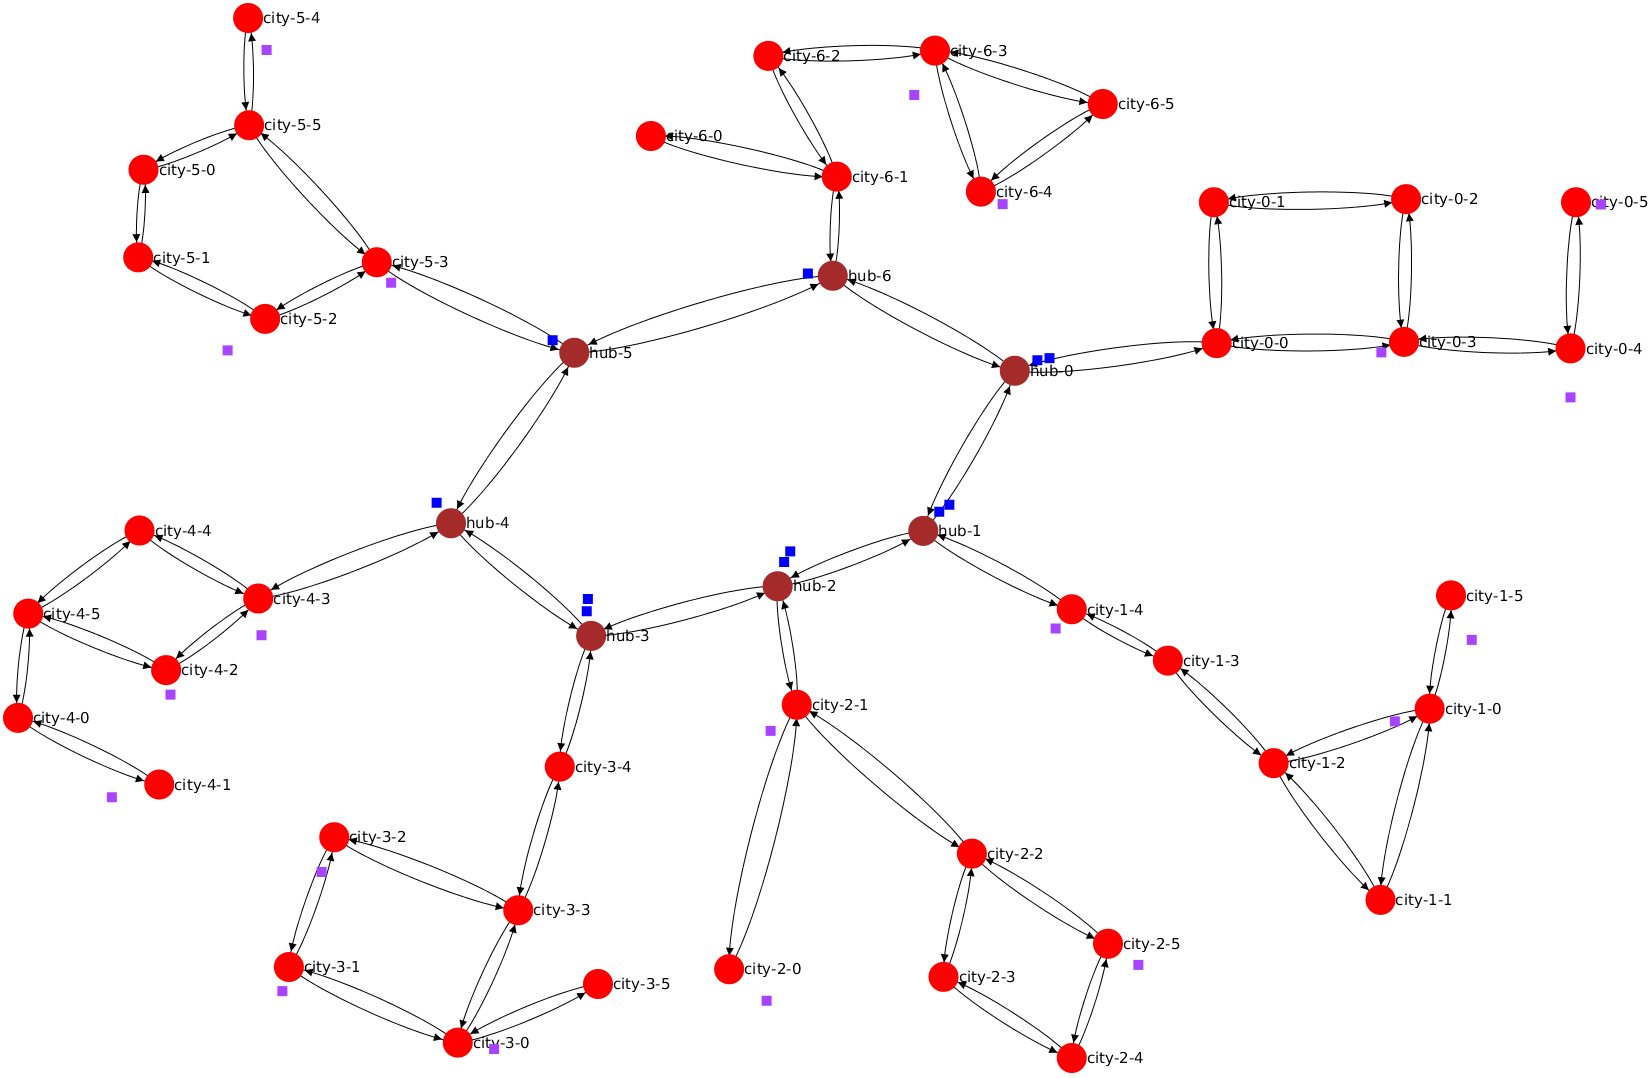
\includegraphics[width=1.0\textwidth]{../img/ipc08_tempo-sat_p30_land}
\end{center}
\caption[Visualization of the \texttt{p30} problem of temporal Transport from IPC 2008.]{Road graph visualization of the \texttt{p30} problem of the tempo-sat track of IPC 2008. Red dots represent locations (graph nodes), roads (graph edges) are represented by black arrows, vehicles are plotted as blue squares, and packages as purple squares. Darker red dots represent locations with petrol stations. In this specific problems, the circle of nodes in the center represents a series of truck hubs and each of the attached subgraphs are individual cities.}
\label{fig:ipc08_tempo-sat_p30}
\end{figure}

\begin{table}[p]
\footnotesize
\centering
\begin{subtable}[t]{0.42\textwidth}
\csvreader[tabular=r||rrrr,
    table head=\textbf{\#} & \rot{\textbf{Vehicles}} & \rot{\textbf{Packages}} & \rot{\textbf{Locations}} & \rot{\textbf{Roads}}\\\midrule\midrule,
    late after line=\mbox{}]
%    table foot=\\\bottomrule]%
{../data/seq-sat-6.csv}{Problem=\problem,Vehicles=\vehicles,Packages=\packages,Locations=\locations,Roads=\roads}%
{\problem & \vehicles & \packages & \locations & \roads}%
\caption{Problem dimensions of the seq-sat-6 dataset.}
\label{tab:seq-sat-6-dims}
\end{subtable}
\quad
\begin{subtable}[t]{0.54\textwidth}
\csvreader[tabular=r||rrrrr,
    table head=\textbf{\#} & \rot{\textbf{Vehicles}} & \rot{\textbf{Packages}} & \rot{\textbf{Locations}} & \rot{\textbf{Roads}} & \rot{\textbf{Petrol}}\\\midrule\midrule,
    late after line=\mbox{}]
%    table foot=\\\bottomrule]%
{../data/tempo-sat-6.csv}{Problem=\problem,Vehicles=\vehicles,Packages=\packages,Locations=\locations,Roads=\roads,PetrolStations=\petrol}%
{\problem & \vehicles & \packages & \locations & \roads & \petrol}%
\caption{Problem dimensions of the tempo-sat-6 dataset.}
\label{tab:tempo-sat-6-dims}
\end{subtable}

\begin{subtable}[t]{1\textwidth}
\vspace{0.5cm}
\begin{subtable}[t]{0.42\textwidth}
\csvreader[tabular=r||rrrr,
    table head=\textbf{\#} & \rot{\textbf{Vehicles}} & \rot{\textbf{Packages}} & \rot{\textbf{Locations}} & \rot{\textbf{Roads}}\\\midrule\midrule,
    late after line=\mbox{}]
%    table foot=\\\bottomrule]%
{../data/seq-sat-8.csv}{Problem=\problem,Vehicles=\vehicles,Packages=\packages,Locations=\locations,Roads=\roads}%
{\problem & \vehicles & \packages & \locations & \roads}%
\end{subtable}
\quad
\begin{subtable}[t]{0.54\textwidth}
\csvreader[tabular=r||rrrr,
    table head=\textbf{\#} & \rot{\textbf{Vehicles}} & \rot{\textbf{Packages}} & \rot{\textbf{Locations}} & \rot{\textbf{Roads}}\\\midrule\midrule,
    late after line=\mbox{}]
%    table foot=\\\bottomrule]%
{../data/seq-sat-8_2.csv}{Problem=\problem,Vehicles=\vehicles,Packages=\packages,Locations=\locations,Roads=\roads}%
{\problem & \vehicles & \packages & \locations & \roads}%
\end{subtable}
\caption{Problem dimensions of the seq-sat-8 dataset.}
\label{tab:seq-sat-8-dims}
\end{subtable}
\caption[Problem dimensions of selected Transport IPC datasets.]{Problem dimensions of selected Transport IPC datasets. Bolded problem instance numbers correspond to Figure~\ref{fig:ipc08_seq-sat_p13} and Figure~\ref{fig:ipc08_tempo-sat_p30} respectively.}
\label{tab:dataset-dimensions}
\end{table}


All sequential problem instances in seq-sat-6 and seq-sat-8 have symmetric roads and road lengths and can, therefore,
be simplified by assuming the use of an undirected graph.
In no sequential problem do vehicles need to finish at a specific target location.

The temporal problems in tempo-sat-6 do not have the same property;
the problems 1--20 have symmetric roads and lengths, but
the 21--30 problems only have symmetric roads, not lengths in general.
The same applies to fuel demands of roads and as a bonus,
these problems have vehicle target locations, which means that not only packages,
but also
vehicles will need to be positioned at specific locations
after package delivery finishes. We can interpret this goal
in a similar way as in a VRP, where a vehicle target location is thought to be
a truck depot or hub. A visualization of such a problem can be seen in Figure~\ref{fig:ipc08_tempo-sat_p30}.

We can see that problems vary not only in size but also in what features they include
and what assumptions they make.
A summary of the acquired insights is available in Table~\ref{tab:problem-properties}.

\begin{table}
\centering
\begin{tabular}{cc||ccccc}
\textbf{Dataset} & \textbf{Problems} & \rot{\textbf{\# of cities}} & \rot{\textbf{Symmetric road lengths}} & \rot{\textbf{Symmetric fuel demands}} & \rot{\textbf{Vehicle target locations}} & \rot{\textbf{State space size}}\\
\midrule
\midrule
\multirow{3}{*}{seq-sat-6} & 01--10 & 1 & \multirow{3}{*}{Yes} & \multirow{3}{*}{N/A} & \multirow{3}{*}{No} & • \\ 
& 11--20 & 2 &  &  &  & • \\ 
& 21--30 & 3 &  &  &  & • \\\midrule%
%
\multirow{6}{*}{seq-sat-8} & 01--03 & 1 & \multirow{6}{*}{Yes} & \multirow{6}{*}{N/A} & \multirow{6}{*}{No} & • \\ 
& 04--06 & 2 &  &  &  & • \\ 
& 07--10 & 3 &  &  &  & • \\ 
& 11--13 & 1 &  &  &  & • \\ 
& 14--16 & 2 &  &  &  & • \\ 
& 17--20 & 3 &  &  &  & • \\\midrule%
%
\multirow{7}{*}{tempo-sat-6} & 01--10 & 1 & Yes & Yes & No & • \\ 
& 11--20 & 2 & Yes & Yes & No & • \\\cmidrule{2-7}
& 21--22 & 3 & \multirow{5}{*}{No} & \multirow{5}{*}{No} & \multirow{5}{*}{Yes} & • \\ 
& 23--24 & 4 &  &  &  & • \\ 
& 25--26 & 5 &  &  &  & • \\ 
& 27--28 & 6 &  &  &  & • \\ 
& 29--30 & 7 &  &  &  & •
\end{tabular} 
\caption{Summary of problem instance properties in IPC Transport datasets.}
\label{tab:problem-properties}
\end{table}

\subsection{Domain insights}

\TODO{Mention heuristics, invariants that hold, try to prove them?}








\section{Accompanying software toolkit architecture}

\TODO{Modules, classes, what belongs where, etc}


















\section{Formulating Transport as a CSP}\label{csp-formulation}

\TODO{intro}

\subsection{Na{\"{i}}ve formulation}

We will now formulate a sequential Transport (Section~\ref{transport-strips}) problem as a CSP (Section~\ref{csp}) using the na{\"{i}}ve encoding provided in \citet[Section~8.3]{Ghallab2004}.
However, using that strategy, our problems ``blow up'' in size --- as is expected due
to the different complexities of planning versus solving CSPs \citep[Section~8.3.2]{Ghallab2004}. To visualize the difference in our case, we have constructed a state space estimation table (Table~\ref{tab:csp-trivial}) for conversions of two sample sequential Transport problems.

\begin{table}[tb]
\begin{center}
\begin{tabular}{l||rr}
\textbf{Features / estimates} & \textbf{p01} & \textbf{p20} \\ 
\midrule
\midrule
\textbf{Best known plan length} & 6 & 351 \\ 
\textbf{Vehicles} & 2 & 4 \\ 
\textbf{Vehicle variables} & 14 & 1 408 \\ 
\textbf{Packages} & 2 & 20 \\ 
\textbf{Package variables} & 14 & 7 040 \\ 
\textbf{Locations} & 5 & 60 \\ 
\textbf{Roads} & 12 & 256 \\
\textbf{Max capacity} & 4 & 4 \\ 
\midrule
\textbf{Ground Drive actions} & 168 & 360 448 \\ 
\textbf{Ground PickUp actions} & 140 & 1 689 600 \\ 
\textbf{Ground Drop actions} & 140 & 1 689 600 \\ 
\midrule
\textbf{Planning variables total} & 48 & 10 207 \\ 
\textbf{Grounded actions total} & 448 & 1 189 838 848 \\ 
\textbf{Search Space Estimate} & $\approx 1.1 \cdot 10^{52}$ & $\approx 1.4 \cdot 10^{27 952}$ \\ % https://www.wolframalpha.com/input/?i=(245120%5E351)+*+4%5E1408+*+60%5E1408+*+1468%5E7040
\end{tabular}
\end{center}
\caption[Search space approximations for a na{\"{i}}ve CSP encoding.]{CSP Search space approximations for the \textit{p01} and \textit{p20} problems from the \textit{seq-sat} track of IPC 2008, using the general and domain-independent encoding from \citet[Section~8.3]{Ghallab2004}.}
\label{tab:csp-trivial}
\end{table}

The first section of the table (rows 1--7) contains problem-specific constants.
The two calculated values in that section, \textit{Vehicle variables} and \textit{Package variables} are the amounts of variables generated for the respective
object by grounding it for every intermediate plan state (before and after applying an action). Therefore, the value is equal to the number of vehicles/packages of the problem
multiplied by the set plan length $+ 1$ (each state corresponds to the state before applying an action + the last state).

In the second section (rows 8--10), we estimate the number of ground actions
Step 1 from \citet[Section~8.3.1]{Ghallab2004} will generate.
We calculate the number of \pickup{} and \drop{} actions the CSP encoding will generate
as $$(\mt{length(plan)} + 1) \cdot \mt{\#vehicles} \cdot \mt{\#locations} \cdot \mt{\#packages},$$
effectively counting all ground planning operators of the problem. Similarly,
the number of \drive{} actions is calculated as
$$(\mt{length(plan)} + 1) \cdot \mt{\#vehicles} \cdot \mt{\#roads},$$
which is more efficient than the na{\"{i}}ve way of
counting all
$$(\mt{length(plan)} + 1) \cdot \mt{\#vehicles} \cdot \mt{\#locations}^2$$
actions.

As we can see from the third section of the table, the number of variables
(planning variables and ground actions) is not extremely high
--- the problem is that the variables have very large domains,
which makes the CSP problem exponentially larger \citep[Section~8.3.2]{Ghallab2004}.
We calculated the \textit{Search Space Size Estimate} (SSE) as
\begin{align*}
\mt{SSE} =\; &\mt{\#ground\_actions}^{l-1} & \textit{\footnotesize select ground actions for the plan}\\
&\cdot \mt{\#capacities}^{l \cdot \mt{\#vehicles}} & \textit{\footnotesize select capacities for vehicle variables}\\
&\cdot \mt{\#locations}^{l \cdot \mt{\#vehicles}} & \textit{\footnotesize select locations for vehicle variables}\\
&\cdot (\mt{\#locations} + \mt{\#vehicles})^{l \cdot \mt{\#pkg}}, & \textit{\footnotesize select locations/vehicles for package variables}
\end{align*}
where we set $l := \mt{length(plan) + 1}$.
For comparison to the SSEs in the last table row, 
the estimated number of atoms in the universe is generally estimated to be about $4 \cdot 10^{80}$.

\subsection{Domain-dependent formulation}\label{csp-custom-repr}

\TODO{domain-dep formulation, note the shadow variable overhead}
\TODO{New cap represents advantages: memory while keeping the same expressive power. Reduction only in state vars}


\begin{table}[tb]
\begin{center}
\begin{tabular}{l||rr}
\textbf{Features / estimates} & \textbf{p01} & \textbf{p20} \\ 
\midrule
\midrule
\textbf{Best known plan length} & 6 & 351 \\ 
\textbf{Vehicles} & 2 & 4 \\ 
\textbf{Vehicle shadow vars} & 14 & 1 408 \\
\textbf{Packages} & 2 & 20 \\ 
\textbf{Package shadow vars} & 14 & 7 040 \\
\textbf{Locations} & 5 & 60 \\ 
\textbf{Roads} & 12 & 256 \\
\textbf{Max capacity} & 4 & 4 \\ 
\midrule
\textbf{Ground Drive actions} & 24 & 1024 \\ 
\textbf{Ground PickUp actions} & 20 & 4800 \\ 
\textbf{Ground Drop actions} & 20 & 4800 \\ 
\midrule
\textbf{Planning variables total} & 48 & 10 207 \\ 
\textbf{Grounded actions in step} & 64 & 10 624 \\ 
\textbf{Action type orderings} & 2 187 & $\approx 8.8 \cdot 10^{167}$ \\ 
\textbf{Search Space Estimate} & $\approx 1.5 \cdot 10^{14}$ & $\approx 2.0 \cdot 10^{637}$ \\
\end{tabular}
\end{center}
\caption[Search space approximations for a domain-dependent CSP encoding.]{CSP Search space approximations for the \textit{p01} and \textit{p20} problems from the \textit{seq-sat} track of IPC 2008, using a custom domain-dependent CSP encoding for Transport sequential.}
\label{tab:csp-custom}
\end{table}

Using the domain-dependent encoding specified previously, we are now able to construct
a search space estimate table for the same Transport problems (Table~\ref{tab:csp-custom}). While the table rows look similar, sections 2 and 3 are calculated
differently. The ground action counts in section 2 are not multiplied by $\mt{length(plan)} + 1$
as done previously, because we only represent them once, not at every plan state.
The total number of grounded actions is the same, but they are not explicitly represented as variables. The Search Space size Estimate is therefore calculated differently:
\begin{align*}
\mt{SSE} =\; &3^{\mt{length(plan)} + 1} & \textit{\footnotesize select the action type of each action}\\
&\cdot \mt{\#ground\_actions}^{l-1}. & \textit{\footnotesize select the specific ground action}
\end{align*}
For comparison to the na{\"{i}}ve encoding SSEs which going from the p01 problem to the p20 grow by a logarithmic factor of approximately $538$,
whereas the domain-dependent ones only grow by approximately $46$,
which is a huge improvement.

Given the search space reduction, we will attempt to use this representation
for constructing a CSP-based planner in Section~\ref{csp-approach}.
